\documentclass[a4paper,english,fleqn]{exam}

\usepackage{babel} % voor nederlandse afbreekregels e.d.
\usepackage{hyperref} % voor links, hier niet gebruikt
\usepackage{graphicx} % voor importeren van figures, hier niet gebruikt
\usepackage{tabularx} % voor tabellen met controle over kolombreedte, hier niet gebruikt
\usepackage{booktabs} % voor nettere tabellen dan de standaard
\usepackage{enumerate} % voor controle over nummering van items
\usepackage{amssymb,amsmath,amsthm,amsfonts} % van de AMS, voor nettere math
\usepackage{qtree} % voor het maken van mooie bomen, hier niet gebruikt
\usepackage{mathabx} %voor het \notdivides commando, niet gebruikt
\usepackage{adjustbox}
\usepackage{listings}
\usepackage{color}
\usepackage{pifont}
\usepackage{algorithm} % pseudocode
\usepackage[noend]{algpseudocode} %pseudocode 
\usepackage{sectsty}

\renewcommand\thesubsection{\thesection \alph{subsection}}
\newcommand{\s}{\text{*}}

%\DeclareGraphicsExtensions{.pdf,.png,.jpg}

\title{Product Planning BEP}

\renewcommand{\baselinestretch}{0.9} 

\sectionfont{\fontsize{11}{15}\selectfont}

\renewcommand{\qedsymbol}{\hfill \emph{QED}}

% document variables:
\newcommand{\cMysename}{Model-based Optimization and Visualization of Aircraft Noise}
\newcommand{\doctitle}{Product Planning }
\newcommand{\deadline}{25 April 2016}
\newcommand{\examdate}{\deadline}
\newcommand{\authors}{Elvan Kula \& Hans Schouten}
% ---

\newcommand{\cmark}{\ding{51}}%
\newcommand{\xmark}{\ding{55}}%

\newcommand{\itab}[1]{\hspace{0em}\rlap{#1}}
\newcommand{\tab}[1]{\hspace{.2\textwidth}\rlap{#1}}

% http://tex.stackexchange.com/questions/110328/formatting-a-logical-pd-derivation:
\newcommand{\fgh}[1]{\fvline%
  \makebox[0pt][l]{{%
      \raisebox{-1.4ex}[0pt][0pt]{\rule{#1}{\arrayrulewidth}}}}%
  \hspace*{\fitchindent}}
  
  \lstset{language=Java,
%alles tussen "//(*" en "*)" wordt als TeX code verIrkt
	escapeinside={//(*}{*)}} 
 


\newcommand*\xor{\mathbin{\oplus}}
% Fill these in:

% if you use algorithms, this is a nice one:
% http://www.lirmm.fr/~fiorio/AlgorithmSty/
%\usepackage[algo2e]{algorithm2e}

\makeatletter

\makeatother

%%%%%%%%%%%%%%%%%%%%%%%%%%%%%%%%%%%%%%%%%%%%%%%%%%%%%%%%%%%%%%%%%%%%%%%%%%%%%%%%
%% document start
%%%%%%%%%%%%%%%%%%%%%%%%%%%%%%%%%%%%%%%%%%%%%%%%%%%%%%%%%%%%%%%%%%%%%%%%%%%%%%%%
\begin{document}
\thispagestyle{empty}

\begin{center}

\vspace*{2cm}
{\huge \cMysename}

\begin{center}
    \line(1,0){450}
\end{center}

{\LARGE \doctitle}

\vspace{1cm}

{\Large \examdate}

\end{center}
\newpage

\tableofcontents
\newpage
%%%%%%%%%%%%%%%%%%%%%%%%%%%%%%%%%%%%%%%%%%%%%%%%%%%%%%%%%%%%%%%%%%%%%%%%%%%%%%%%
%% end of front page
%%%%%%%%%%%%%%%%%%%%%%%%%%%%%%%%%%%%%%%%%%%%%%%%%%%%%%%%%%%%%%%%%%%%%%%%%%%%%%%%

\section{Introduction}

The goal of our project is to create a standalone software application which can be used by researchers from the Air Transport \& Operations department at TU Delft for model-based optimization and visualization of aircraft noise. To achieve a good development process and a successful software product careful planning is required.

In the second chapter of this document an analysis of our program is provided by describing the context, problem and stakeholder inputs. Based on this the features needed for the product are described in a high level backlog and the steps needed to complete the project are defined in a roadmap. Here you can find the major release schedule and goals.

Chapter 3 contains a detailed release plan specifying our milestones per release. In chapter 4 a definition of 'done' is given on backlog items, sprints and releases. This will enable us to know when a feature is done and when the corresponding sprint item can be closed. 

\section{Product}

This chapter gives a high level overview of the product. Paragraph 2.1 gives a brief analysis of the program and high level overview of the product backlog. In paragraph 2.2 the steps needed to create this program will be described in a roadmap of major releases. Here the major releases of the program are given in a clear overview.

\subsection{Program Overview}

\textbf{Analysis context} \\
Aircraft and airport noise are complex subject matters which have been studied for decades and are still the focus of many research efforts nowadays. Also at the department of Air Transport \& Operations (ATO) at TU Delft’s Faculty of Aerospace Engineering. ATO has three research aims: 1) To develop radical new ways to optimise aircraft operations for efficiency, safety, cost and environmental impact; 2) To extend the analysis to an airline fleet and network level to include capacity and resilience; 3) To synthesize these to include operational safety at an airline and ATM level. To support their research findings at conferences, they need a visualization application that does this.

\textbf{Analysis problem} \\
The ATO research department needs a program that represents a creative and efficient way to minimize and visualize aircraft noise along simulated and real flight routes. This requires the implementation of a mathematical model for aircraft noise and aircraft trajectory design. The model will be deployed by the research team to predict aircraft noise along a particular trajectory (flight route) in order to be able to minimize the produced noise over populated areas around airports. In order to implement this model the parameters that are required for the sound calculation need to be derived mathematically. Besides that, the program should also be able to visualize the noise produced along the simulated trajectory pictured on a real map. This requires an implementation of noise contours, which are ‘noise footprints’ whose shape indicate areas of constant noise. Noise contours are a new subject to the research group and haven’t been implemented in relation with optimization regarding noise reduction before so this will be a challenging topic. The visualization should also show the effects of the produced aircraft noise on population annoyance.

\textbf{Analysis stakeholder inputs} \\
The application needs to be able to read in two arbitrary data (.dat extension) or text files indicating the input trajectory (including selected airplane model) and the grid that needs to be used. These files will be given as input to the sound model. The sound model will then calculate the noise levels produced along the trajectory and the output of the sound model will be entered into the optimization model or will directly be sent to the visualization component.

Additionally, the stakeholder will deliver us some papers and extra explanation on the mathematical concepts behind the optimization model and contouring algorithm. 

\textbf{Product requirements} \\
Our product should be able to do the following tasks:

\begin{itemize}
\item Optimize the existing sound model with multi-core processing to achieve real-time performance.
\item Calculate and output the actual noise contours produced along the input trajectory
\item Optimize the input trajectory based in order to reduce the produced noise 
\item Visualize the optimized trajectory together with the noise contours in real-time 3D animation mapped on Google Earth
\item Calculate and visualize the effects of produced noise on population annoyance using the awakenings algorithm
\item Save the results in a particular format and directory specified by the user
\item It should be possible to perform all these tasks in a graphical user interface
\end{itemize}

\newpage 

\subsection{Roadmap}
In the roadmap below major releases of the program are spread across different phases of software development and they are given in a clear overview. \\

\begin{figure}[ht]
    \centering
    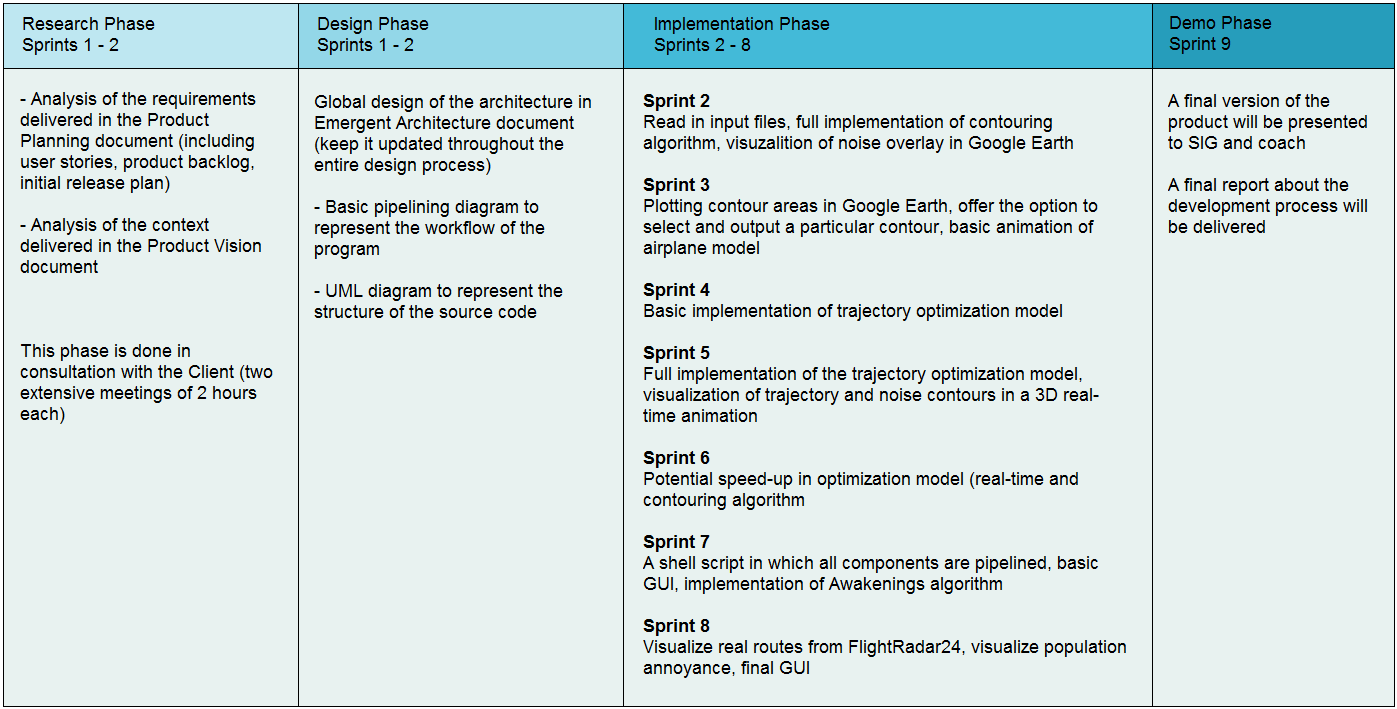
\includegraphics[width=1.1\textwidth]{images/roadmap}
\end{figure}
\section{Product Requirements}

This chapter describes the requirements of our program. The first subsection gives the user stories of the features that need to be implemented. The second subsection focuses on technical issues found in existing products of competitors which will be solved in our product. The third subsection describes the user stories for the knowledge acquisition. The last subsection shows an initial release plan with milestones. 

\subsection{User stories of features}
In this paragraph the user stories of features are sorted by priority using the MoSCoW method:

\textbf{Must have} \\ 
These features are must haves since the program would not be functioning and meet the (minimal) requirements of the customer without these implemented. 

\begin{itemize}
\item As an ATO researcher, I want to read in an arbitrary data file (.dat extension) or text file indicating the input flight trajectory and grid (based on the RD-coordinate system) that I select from a directory.
\item As an ATO researcher, I want to export the resulting animation as a KML file so that I can also run the animation later in Google Earth without needing to start all over again. 
\item As an ATO researcher, I want the sound model to calculate four types of noise levels: A-Weighted Sound Exposure Level (SEL), Effective Perceived Noise Level (EPNL), A-Weighted Maximum Sound Level (LAMAX) and Tone-Corrected Maximum Perceived Noise Level (PNLTM). This should be done conform world standards following the AC Model.
\item As an ATO researcher, I want to calculate noise contours (contour area) produced along the input trajectory using noise input data based on six possible noise metrics: single event metrics (SEL, LAMAX, EPNL, PNLTM) and cumulative noise metrics (Day-Evening-Night Average Level $L_{DEN}$, Night Average Level $L_{night}$). This should be done automatically after the noise model has finished calculating the noise levels.
\item As an ATO researcher, I want to export the actual contour data as a text file or .dat file so that I can save the results in a directory. 
\item As an ATO researcher, I want to optimize the input flight trajectory within the International Standard Atmosphere using a dynamic optimization algorithm based on three models: operational constraints (depending on the used aircraft model), noise model (depending on calculated noise contours) and geographical model. If I select the option to optimize, this calculation should be done automatically by the application after the contouring algorithm has been performed.
\item As an ATO researcher, I want to visualize the input flight trajectory and the produced noise contours in a real-time 3D animation mapped on Google Earth.
\item As an ATO researcher, I want a modern and easy-to-use interface to select files, select the contour(s) I am interested in, select the output that needs to be produced (optimization and/ or visualization) and select a directory to store the output.
\end{itemize}

\newpage

\textbf{Should have}

These features are should haves since the basic components of the program would work without these features but it would be better (meet the requirements of the customer better) if these would be implemented. 

\begin{itemize}
\item As an ATO researcher, I want the sound model to perform real-time.
\item As an ATO researcher, I want to be able to disrupt or cancel the noise, optimization or visualization operations in case I made a mistake and want to change my input data.
\item As an ATO researcher, I want to be able to select a real flight route from the tool FlightRadar24 and visualize this with its calculated noise contours in a real-time 3D animation in Google Earth.
\end{itemize}

\textbf{Could have} \\
These features are could haves since they are not necessary to the customer and to the functioning of the program but it would be nice to include them if there is enough time left in our timeframe. 

\begin{itemize}
\item As an ATO researcher, I want to be able to perform adjustments to the input data in case a data element needs to be changed or added. 
\item As an ATO researcher, I want to have the option to transform the coordinates of my input grid if they are not based on the RD-coordinate system that is required by the noise model.
\item As an ATO researcher, I want to read in Matlab and Excel output files.
\item As an ATO researcher, I want the GUI to show me (real time) how much progress is made in the analysis of the data so that I can estimate how long I have to wait for the results.
\item As an ATO researcher, I want to call the program by a name and recognise it by its logo so that I can share it with others.
\end{itemize}

\textbf{Won't have} \\
These features are won't haves since the customer doesn't actually need these features to be implemented. There probably won't be enough time left for the following features but it could be interesting for a follow-up phase of the project. 

\begin{itemize}
\item As an ATO researcher, I want a logger to log all the operations I have done in the program so that I can have an overview of the input files I entered and visualized. 
\item As an ATO researcher, I want to add comments to certain parts of the input data such as data elements and data chunks so that I can make memos of my own reflections on the data.
\end{itemize}

\newpage
\subsection{User stories of technical improvements}
\textbf{Must have} \\
This feature is a must have since it's a main shortage in existing software that the client uses. This technical improvement would be a unique selling point for our program. 
\begin{itemize}
\item As an ATO researcher, I want the program to perform the noise model, optimization model and visualization model in a pipelined fashion and automated manner without me needing to perform any actions (after the input data is entered).
\item As an ATO researcher, I want the program to optimize input trajectories using the contour data and not just the noise data (this algorithm hasn't been implemented before).
\end{itemize}

\textbf{Should have} \\
These features are should haves since their improvement would add (new) functionality to the program but they are not necessary for the customer. 
\begin{itemize}
\item As an ATO researcher, I want the program to be easier to use than the existing NOISHHH tool (noise model) and NoiseLAss program (optimzation model) so that I don't need to spend much time on configurations and learning how to use the program.
\end{itemize}

%maak nieuwe subsection hiervan in research report
%\subsection{User stories of know-how acquisition}
%This paragraph describes which documents we need to read in order to build the background knowledge that is required to make a future technical decision or precise scheduling based on the user's needs. 

%We need to read about the following subjects:
%\begin{itemize}
%\item As an ATO researcher, I want the development team to read the technical manual INM 7.0 for the integrated noise model which represents the algorithms and methodology used to compute noise-level and time-based metrics based upon finite flight-segment data. They can also use this noise tool to validate their results in case they decide to improve the noise model for speed-up.
%\item As an ATO researcher, I want the development team to read about the contouring algorithm described in the documentation about the noise assessment tool NoiseLAss. This document explains the general algorithm and the way b-spline interpolation can be used to make contour areas more smooth.
%\item As an ATO researcher, I want the development team to read about the Awakenings algorithm (also described in the NoiseLAss documentation) which provides formulas on the calculation of population annoyance caused by aircraft noise.
%\item As an ATO researcher, I want the development team to read about the existing trajectory optimization tool NOISHH and the dynamic optimization algorithm it uses (described in Joeri Dons' MSc thesis: 'Optimization of Departure and Arrival Routing for Amsterdam Airport Schiphol'). This way they will understand how to optimize trajectories regarding to the produced noise contours. They can also use this optimization tool to validate their results. 
%\end{itemize}

\newpage 

\subsection{Initial release plan (milestones, MRFs per release)}
The milestones are spread across different sprints and described below with the corresponding goals. All the releases are continually tested with system testing throughout the entire project. Please note that a sprint corresponds with one week.

\textbf{Sprint 1: 18/04/2016 - 24/04/2016 } \\
This release will contain at least the following features:
\begin{itemize}
\item A Product Planning document containing a roadmap, overall planning and user stories that are prioritized in consultation with the client.
\item A set-up of the Emergent Architecture document containing a pipeline diagram representing the workflow of our program and the way in which the noise, optimization and visualization models are connected.
\end{itemize}

\textbf{Sprint 2: 25/04/2016 - 01/05/2016 } \\
This release will contain at least the following features:
\begin{itemize}
\item A Research Report in which the problem, context and possible solutions are analysed. This will be discussed with the client.
\item An implementation of the contouring algorithm (refining the grid, finding switch points and clustering points with a similar noise level)
\item An implementation of the algorithm that converts Rijksdriehoekscoördinaten to WGL coordinates (long/lat)
\item Basic visualization of noise contours with an overlay on Google Earth
\end{itemize}

\textbf{Sprint 3: 02/05/2016 - 08/05/2016} \\
This release will contain at least the following features:
\begin{itemize}
\item Extended visualization of the noise contours plotted/ mapped in Google Earth
\item An implementation of the spline interpolation algorithm to smoothen out the contour lines
\item The option to output actual noise data
\item The option to turn on or off particular noise contours in the visualization
\end{itemize}

\textbf{Sprint 4: 09/05/2016 - 15/05/2016} \\
This release will contain at least the following features:
\begin{itemize}
\item Basic implementation of the trajectory optimization model (point-mass calculation)
\end{itemize}

\textbf{Sprint 5: 16/05/2016 - 22/05/2016} \\
This release will contain at least the following features:
\begin{itemize}
\item Full implementation of the trajectory optimization model (added: operational constraints)
\item Visualization of the input trajectory and noise contours in a 3D real-time animation in Google Earth (link all visualization components together)
\end{itemize}

\textbf{Sprint 6: 23/05/2016 - 29/05/2016} \\
This release will contain at least the following features:
\begin{itemize}
\item Speed-up in the trajectory optimization model (real-time)
\item Potential speed-up of the contouring algorithm
\end{itemize}

\textbf{Sprint 7: 30/05/2016 - 05/06/2016} \\
This release will contain at least the following features:
\begin{itemize}
\item A shell script in which all operations are pipelined and performed in an automated manner
\item First version of the GUI containing containing a menu bar and tabs for the import of files, noise model (with raw noise level data as output) and optimization model.
\item An implementation of the Awakenings algorithm to calculate population annoyance
\item Emergent Architecture document presenting the final state of the architecture design. 
\end{itemize}

\textbf{Sprint 8: 06/06/2016 - 12/06/2016} \\
This release will contain at least the following features:
\begin{itemize}
\item The option to insert a real flight route from FlightRadar24 and visualize this with a 3D animation in Google Earth
\item Final version of the GUI representing the three models (noise, optimization, visualization) and all possible user operations (added: visualization tab).
\item A visualization of population annoyance in Google Earth (linked with the animation)
\end{itemize}

\textbf{Sprint 9: 13/06/2016 - 19/06/2016} \\
This release will contain at least the following features:
\begin{itemize}
\item Solved bugs and other problems from the previous sprint(s).
\item Final product containing at least all must-have and should-have requirements.
\item Final report about the developed, implemented, and validated software product.
\end{itemize}
\subsection{Definition of Done}
This chapter describes the definition of done so that we both will have the same end goals. This will enable us to know when a feature is done and when the corresponding sprint item can be closed.

Our definition of done focuses on three levels: backlog items (features), sprints and releases.

\textbf{4.1 Level 1: Backlog items} \\
We consider a backlog item as done when it has an test coverage of at least 75\% for non-GUI elements. These tests can be divided into unit tests and other automated tests. For a feature to be merged (using a pull request) into the release version of the product, it has to be approved by the other team member. Their approval will be based on the test coverage, code readability, documentation and the overall code quality. Documentation should be added on every class and method. 

\textbf{4.2 Level 2: Sprints} \\
Every sprint corresponds to one week. At the end of a sprint, all the items on the sprint plan of the current sprint have to be finished, according to the definition of done for backlog items. A new release of our product should be submitted to the version control server (Github) master. All the unit tests should pass and the system should be improved based on added or extended features. There shouldn't be any bugs/errors left in the system and the program should behave and look like the client wanted. We should also have written a sprint reflection for that sprint and a new sprint plan for the coming sprint. 

\textbf{4.3 Level 3: Releases}\\
A release version of our product is done at the end of a sprint. The release version should contain the features that should have been implemented for the corresponding sprint. This also includes the minimal test coverage and other conditions described in the definition of done for a sprint. It is also important to note that the potential feedback of the client for that week should be processed before a release is completed.
In the final release we should have implemented all must haves since the program can't function without these mandatory features. Most should haves (50 to 60\%) and some could haves (30 to 40\%), which are defined in 3.1, have to be implemented. As explained in chapter 3, these features are not necessary for the user and the system to work but our goal is to implement them partially since it would be nice to include them. It would make our program more user friendly. 
Lastly, the final release and other major releases should be approved by the client, the coach and obviously by ourselves too. This means that it should be simple and efficient to use for the client and well documented and designed by us. The SIG test is also an important part of this. They will determine if the code meets the standards and if it is clearly structured and documented. 

As developers we also strive for maintainability and extendability, so that the system can be easily maintained, improved and updated by us or other people after our final release. This will also be taken into account throughout the entire project.

% completion of project: binaries, packaging of the project 




\end{document}
%%%%%%%%%%%%%%%%%%%%%%%%%%%%%%%%%%%%%%%%%%%%%%%%%%%%%%%%%%%%%%%%%%%%%%%%%%%%%%%%